 

\actTitle{Worksheet 1.1}

\videoLink{Section 1.1}{https://www.youtube.com/playlist?list=PLYHZK3b8UFw3ad1wlhTMGcL5kgita6QGS}

\noindent
Student goals:
  \begin{itemize}
  \item Plot points in the coordinate plane.
  \item Identify the four quandrants of the coordinate plane.
  \item Calculate the distance between two points.
  \item Make rough sketch of the graph of a function by plotting
    points first.
  \item Determine the $x$ and $y$ intercepts of a function
    analytically and graphically.
  \end{itemize}


\noindent \textbf{Instructions:}  Work together in groups of  3 or 4 to complete the following problems.


\begin{enumerate}

\item Mark the points $P_1(-2,-4.5)$ and $P_2(4,1.5)$ on the
  coordinate plane below. Determine the distance between the two
  points.  Include a sketch of a right triangle whose hypotenuse
  represents the distance between the two points. Label the lengths of
  each side of the right triangle, and for each point state which
  quadrant it lies in.

  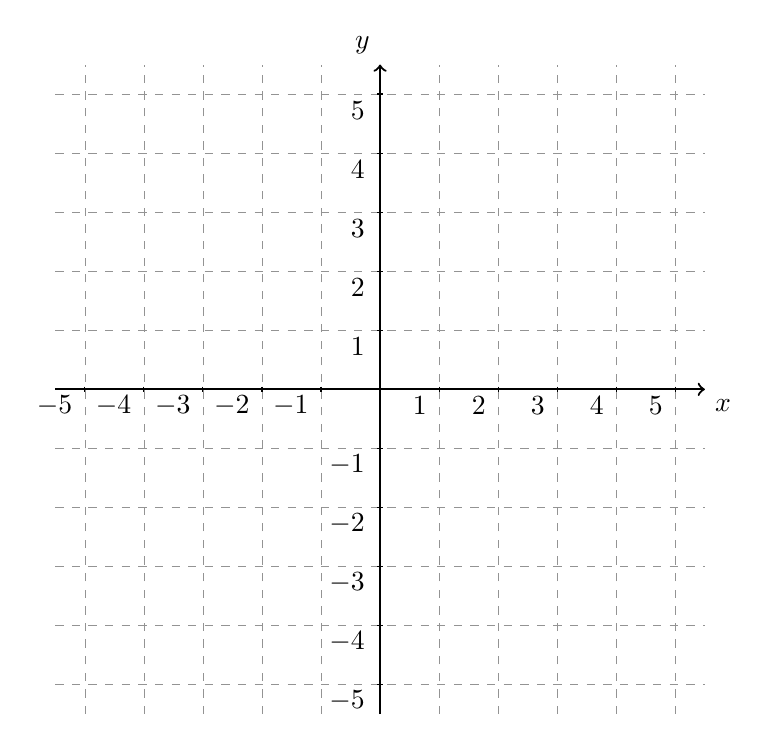
\begin{tikzpicture}[y=0.75cm, x=0.75cm,font=\sffamily]
    % bounds
    % ticks
    \draw[step = 1, gray, very thin,dashed,opacity=0.85] (-5.5, -5.5) grid ( 5.5,5.5);
 	% axis
	\draw[thick,->] (-5.5,0) -- coordinate (x axis mid) (5.5,0) node[anchor = north west] {$x$};
    \draw[thick,->] (0,-5.5) -- coordinate (y axis mid) (0,5.5) node[anchor = south east] {$y$};
    \foreach \y in {-5,-4,...,-1,1,2,...,5.5} {
      \draw (1pt, \y) -- (-1pt, \y) node[yshift=-6,xshift=-1,anchor=east] {$\y$};
    }
    \foreach \x in {-5,-4,...,-1,1,2,...,5.5} {
      \draw (\x,1pt) -- (\x,-1pt) node[yshift=-5,xshift=-1,anchor=east] {$\x$};
    }
  \end{tikzpicture}


\clearpage


\item Determine the $x$ and $y$ intercepts of the following equations.
\begin{enumerate}
\item $x^2+y=9$
  \vfill
\item $y=|x+4|-3$
  \vfill
\end{enumerate}

\item Each of the questions below refers to the equation
  \begin{eqnarray*}
    y & = & |x-2| + h,
  \end{eqnarray*}
  where $h$ is a real number.
  \sideNote{Assume a point is an $x$-intercept and then ask what it
    implies about the resulting equation.}
  \begin{enumerate}
  \item Suppose you know that the graph of the equation has two
    $x$-intercepts. What does this imply about the possible values
    that $h$ could be?
    \vfill
  \item Suppose, instead, you know that the graph of the equation has
    one $x$-intercept. What does this imply about the possible values
    that $h$ could be?
    \vfill
  \item Suppose, instead, you know that the graph of the equation has no
    $x$-intercept. What does this imply about the possible values
    that $h$ could be?
    \vfill
  \end{enumerate}

\clearpage

\item Determine all points lying on the $y$-axis that are 5 units away
  from the point $(4,-2)$.  Use the problem solving process stated
  below, and explicitly identify which part of the process you are
  using in each of your steps.  As a group, write your complete
  solution on the board.


\begin{boxthm}
{\bf Problem Solving Process}
\begin{enumerate}
\item Re-read the problem.
\item Determine what the problem is asking for along with the format of that answer.
\item Circle/Underline the important components of the problem.
\item Determine the topics/concepts being assessed.
\item Write down relevant formulas, definitions, and equations.
\item Discuss your ideas with your group.
\item Make rough sketches of the relationships and try to visualize
  the situation and context.
\item Solve the problem and verify that your solution answers the
  question in the correct format.
\end{enumerate}

\end{boxthm}
\vfill
\clearpage

\item A turtle is in a field. Initially, it is 40 meters north and 60
  meters west of the center of the field.
  \begin{enumerate}
  \item What is the turtle's distance from the center of the field?
    (Make a sketch of the situation using a coordinate system and
    label the axes and important aspects of the graph.)

    \vfill
    \vfill
    
  \item The turtle is moving at a constant speed, and it moves east
    one meter per minute. How far does it move from its initial
    position in $t$ minutes?
    
    \vfill
    
  \item Describe what happens to the turtle's distance from the center
    of the field as time goes by. Do not give an exact answer but give
    a general description of the important trends over time. What
    happens to the distance after a long time?
    
    \vfill

  \item Make a rough sketch of the distance based on your
    description. \sideNote{The graph should not be exact but just
      roughly conveys the important features.}

    \vfill
    \vfill

  \item What is the turtle's location when the distance from the
    center of the field is at its smallest? Are there any times when
    the distance from the center of the field is unique? (i.e. there
    are no other times when the distance is the same.)

    \vfill
    
  \end{enumerate}



\end{enumerate}




\hwTitle{Section 1.1}

\begin{enumerate}
\item The points $ABC$ form a triangle.
  \begin{enumerate}
  \item Plot $A(-1,2),B(3,0) , C(4,2), $ and draw the triangle on the graph below.\\
    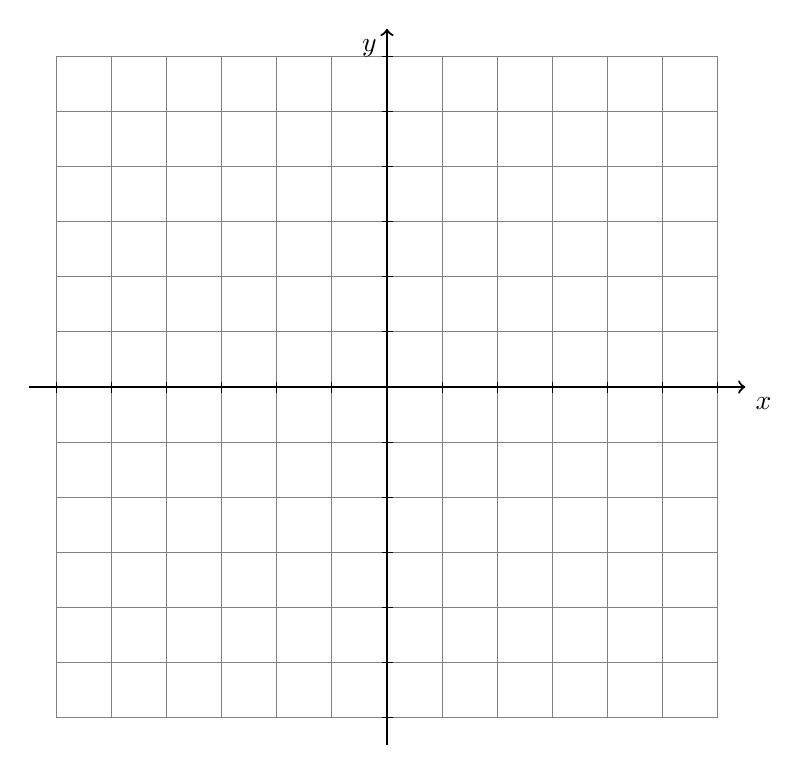
\begin{tikzpicture}[y=.7cm, x=.7cm,font=\sffamily]
      %% ticks
      \draw[step = 1, gray] (-6,-6) grid (6,6);
      %% axis
      \draw[thick,->] (-6.5,0) -- coordinate (x axis mid) (6.5,0) node[anchor = north west] {$x$};
      \draw[thick,->] (0,-6.5) -- coordinate (y axis mid) (0,6.5) node[anchor = north east] {$y$};
      \foreach \y in {-6,-5,...,-1,1,2,...,6} {
        \draw (2pt, \y) -- (-2pt, \y);
      }
      \foreach \x in {-6,-5,...,-1,1,2,...,6} {
        \draw (\x,2pt) -- (\x,-2pt);
      }

    \end{tikzpicture}

  \item Determine the perimeter of the triangle.
  \item Is the triangle a right triangle?  Show work to support your answer.
  \end{enumerate}

\item Use the following parts to find all points on the line $y=2x$ that are 5 units away from $P(-1,3)$.  
  \begin{enumerate}
  \item Find the points $(x,y)$ on the line $y=2x$ for $x=1, -2,$ and $5$.
  \item What if we didn't know the value of $x$?  Write an ordered
    pair formula that works for every point on the line $y=2x$?
  \item Use part (b) to find all points on the line $y=2x$ that are 5 units away from $P(-1,3)$. 
  \end{enumerate}


\item Determine the $x$ and $y$ intercepts of the following equations.
  \begin{enumerate}
  \item $\displaystyle y=3x+10.$
  \item $\displaystyle y=\sqrt{x-10}.$
  \item $\displaystyle y^2 = (x-4)^2.$
  \item $\displaystyle y = x^3 - x.$
  \item $\displaystyle |y-3| = 2|x+1| + 5.$
  \end{enumerate}

\item For each equation below determine all possible values of $x$
  that can be used to calculate a valid value of $y$. Express your
  result three different ways, using interval notation, graphically on
  a line segment, as well as using inequalities.
  \begin{enumerate}
  \item $\displaystyle y=|x+10|.$
  \item $\displaystyle y=\frac{3}{4-x}.$
  \item $\displaystyle y=2x+19.$
  \item $\displaystyle y = \sqrt{x+5}.$
  \item $\displaystyle y = \frac{10}{\sqrt{x+5}}.$
  \end{enumerate}

\item The Racine express is moving straight North out of Chicago, and
  the Davenport Traveler is moving straight West out of Chicago. At a
  given point in time the distance between the trains is four-hundred
  and fifty miles. If the Racine express is ninety miles North of
  Chicago determine the coordinates of the other train. (Treat Chicago
  as the origin.)

\item A rabbit is located in the center of a field. The rabbit's
  burrow is located 20 meters north and 30 meters east of where it is
  currently located. A fox is located 25 meters north and 37 meters
  east of the burrow. If the rabbit can run 11 meters per second and
  the fox can run 13.6 meters per second, can the rabbit reach its
  burrow before the fox reaches the burrow assuming they start running
  at the same time? (Make a sketch of the situation and clearly mark
  the positions of each relevant object.) The time it takes for an
  object moving at a speed of $v$ meters per second to travel $d$
  meters is $\frac{d}{v}$.

  The time it takes for an object moving at a velocity $v$ kph to travel
  $d$ meters 

  \item Mark the point $P_3(1.3,-2.4)$ on the coordinate plane below. Determine the
  points on the $x$-axis that are a distance of 3 units from $P_3$.

  \begin{tikzpicture}[y=1cm, x=1cm,font=\sffamily]
    % bounds
    \def\lowX{-5.5}
    \pgfmathtruncatemacro\startX{round(0.5+\lowX)}
    \pgfmathsetmacro\nextXValue{int(\startX+1)}
    \def\highX{5.5}
    \def\lowY{-5.5}
    \def\highY{5.5}
    \pgfmathsetmacro\nextYValue{int(\lowY+1)}
    % ticks
    \draw[step = 1, gray, very thin,dashed,opacity=0.85] (\lowX, \lowY) grid ( \highX,\highY);
 	% axis
	\draw[thick,->] (\lowX,0) -- coordinate (x axis mid) (\highX,0) node[anchor = north west] {$x$};
    \draw[thick,->] (0,\lowY) -- coordinate (y axis mid) (0,\highY) node[anchor = south east] {$y$};
    \foreach \y in {-5,-4,...,-1,1,2,...,\highY} {
      \draw (1pt, \y) -- (-1pt, \y) node[yshift=-6,xshift=-1,anchor=east] {$\y$};
    }
    \foreach \x in {-5,-4,...,-1,1,2,...,\highX} {
      \draw (\x,1pt) -- (\x,-1pt) node[yshift=-5,xshift=-1,anchor=east] {$\x$};
    }
  \end{tikzpicture}

  \begin{subproblem}
  \item Place points on the graphs near to where you think the points
    \textbf{may} be located.
  \item Label one of the points, $(x,y)$. 
  \item Write out the general distance formula.
  \item What do you know about the point? Can you simplify the formula?
  \item Solve for the unknown variable.
  \end{subproblem}

\end{enumerate}
